\setcounter{page}{8}

\fontsize{10}{14pt}\selectfont

\begin{multicols}{2}
\noindent имеем

\begin{align}
    \noindent \left| xy \right| =\left| (ma+nc)(\frac{m}{a}-\frac{n}{c}) \right| = \left| m^{2} +mn (\frac{c}{a}-\frac{a}{c})-n^{2} \right| = \\ = \left| m^{2} +mn-n^{2}\right|
\end{align}

Внутренность «креста» из гипербол \(xy = \pm 1\) задается неравенством \(|xy| < 1\). Но при целых \textit{m} и \textit{n} величина \(\left| m^{2} + mn - n^{2} \right|\) тоже целая. Единственным целым числом, которое по модулю меньше 1, является ноль.

\setcounter{figure}{3}

\begin{wrapfigure}{l}{0.6\linewidth}
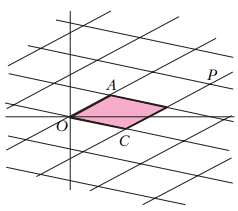
\includegraphics[width=150px]{image.png}
\caption{}
\end{wrapfigure}

\noindent Значит, для лежащей внутри креста точки решетки имеем откуда \(ma + nc = 0\) или \(mc – na = 0\). Ввиду иррациональности отношения \(a/c\) это возможно лишь при \(m = n = 0\).

Значит, внутри «креста» из гипербол расположена единственная точка
рассматриваемой решетки – начало координат.

Для решетки, порожденной параллелограммом рисунка 3, решение аналогично, поэтому мы выпишем только формулы
\[\overrightarrow{OP} = m\overrightarrow{OA} + n\overrightarrow{OC} = (ma + nc; \frac{m}{a} + \frac{n}{c})\]
и

\begin{align}
    \noindent \left| xy \right|=\left| (ma+nc)(\frac{m}{a}+\frac{n}{c}) \right| = | m^{2}+mn(\frac{c}{a}+\frac{a}{c}) + +n^{2} |= \\ = \left| xy \right|=\left| (ma+nc)(\frac{m}{a})+\frac{n}{c} \right| = \\ =\left| m^{2}+mn(\frac{c}{a}+\frac{a}{c})+n^{2} \right|=\left| m^{2}-3mn+n^{2} \right| = \\ = \left| (m-n)^{2}-(m-n)n-n^{2}) \right|=\left| k^{2} - kn - n^{2} \right|, \text{где обозначено} k= \\ =m-n\\
    
\end{align}

Итак, внутри «креста гипербол» нет ни одной точки решеток, кроме начала координат. А на самих гиперболах таких точек бесконечно много. Чтобы доказать это, в первом из рассмотренных нами случаев достаточно убедиться, что уравнение

\[m^{2} + mn - n^{2} = \pm 1\]
имеет бесконечно много решений в целых числах \textit{m}, \textit{n},
а во втором случае – сделать то же самое для уравнения
\[k^{2} - kn - n^{2} = \pm 1\]
Впрочем, первое из этих двух уравнений сводится ко
второму заменой m на –k.

\begin{center}
\textbf{Уравнение:} $\bm{x^2 - xy - y^{2} = \pm 1}$
\end{center}

Это уравнение не имеет вида \(x^{2} - dy^{2} − = 1\). Но умножение на 4 приводит его к виду

\[4x^{2}-4xy-4y^{2}=\pm 4,\]

\noindent т.е.

\[(2x-y)^{2}-5y^{2}=\pm4\]
что уже похоже на уравнение Пелля. Впрочем, мы
воспользуемся этим преобразованием чуть позже, а
здесь решим уравнение в его первоначальном виде.

Немного посчитав, можно составить таблицу:

\begin{table}{0.2}{c\linewidth}
\centering
\begin{tabular}{|c|c|c|c|c|c|c|c|c|c|}

\end{tabular}
\end{table}

\setlength\extrarowheight{3pt}    
{\centering
\begin{tabular}{|c|c|c|c|c|c|c|c|c|c|}
\hline
    \textit{x} & 0 & 1 & 1 & 2 & 3 & 5 & 8 & 13 & 21 \\
    \hline
    \textit{y} & 1 & 0 & 1 & 1 & 2 & 3 & 5 & 8 & 13 \\
    \hline
    x^2 - xy -y^2 & -1 & 1 & -1 & 1 & -1 & 1 & -1 & 1 & -1 \\
\hline
\end{tabular}
}
\vspace{0.35cm}

Всякий, кто знаком с числами Фибоначчи, уже узнал. А остальным скажем, что последовательность Фибоначчи задана своими двумя членами \(\varphi_{0} = 0\), \(\varphi_{1} = 1\) и \texttt{рекуррентной формулой} \(\varphi_{n+2} = \varphi_{n} + \varphi_{n+1}\). Несколько следующих членов этой замечательной последовательности таковы: \(\varphi_{2} = 0+1=1, \ \varphi_{3} = 1+1=2, \ \varphi_{4} = 1+2 = 3, \ \varphi_{5} = 2+3=5, \ \varphi_{6} = 3+5=8, \ \varphi_{7} = 5+8=13\).

\textbf{Теорема 6.} \textit{Если} \(x^{2} - xy - y^{2} = \pm 1\), \textit{то пара чисел}
\((X;Y) = (x + y; x)\) \textit{удовлетворяет равенству} \(X^{2} - XY - Y^{2} = \mp 1 \).

\textbf{Доказательство.}

\begin{multline*}
(x+y)^{2} - (x+y)x-x^{2}=x^{2}+2xy+y^{2}-x^{2}- -xy-x^{2}= -(x^{2}-xy-y^{2})=\mp 1.
\end{multline*}

Доказав теорему 6, мы наконец-то решили задачу М1775.

Как и не раз выше, сформулируем и не докажем еще одну теорему.

\textbf{Теорема 7.} \textit{Уравнение} \(x^{2} - xy - y^{2} = \pm 1\) \textit{не имеет решений в целых неотрицательных числах, кроме тех, что получаются из «тривиального» решения} (0;1) при помощи правила \((x;y) \to  (x+y;x).\)

\textbf{Следствие.} Все решения уравнения \(z^{2}-5y^{2}=\pm 4\) натуральных числах даются формулой \((z;y) = \varphi_{n+1} + \varphi_{n-1}; \varphi_{n}\).

\textbf{Доказательство.} Каждой паре целых чисел \((x;y)\), удовлетворяющей равенству \(x^{2} - xy - y^{2} = \pm 1\), соответствует пара целых чисел \((z;y)=(2x-y;y)\), удовлетворяющая равенству \(z^{2}-5y^{2}=\pm 4\), и наоборот (поскольку числа \(z\) и \(y\) одной четности). Осталось заметить, что если \(x = \varphi_{n+1}\) и \(y = \varphi_{n}\), то

\[z=2x-y=2\varphi_{n+1}-\varphi_{n}=\varphi_{n+1}+\varphi_{n-1}\]

\textbf{Упражнение 20.} Докажите тождества

\noindent a) \(\varphi^{2}_{n} = \varphi_{n-1}\varphi_{n+1}-(-1)^{n}\);

\noindent б) \(\varphi^{2}_{n} = \varphi_{n-2}\varphi_{n+2}+(-1)^{n}\).

\begin{center}
    (\textit{Продолжение следует})
\end{center}

\end{multicols}
